\begin{center}
    \Huge{\textbf{\underline{Chapter 1: Introduction}}}
\end{center}

\setcounter{section}{0}

\vspace{0.35cm}


\section{Compiler}

\begin{prettyBox}{Definition}{myblue}
A compiler is a software program that takes a piece of code as input, analyzes
it for errors, and generates output in the form of messages or logs.
Additionally, it produces an executable file that can be run on a computer.
\end{prettyBox}

\vspace{0.35cm}
\begin{center}
    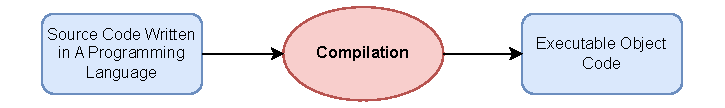
\includegraphics[width=0.8\textwidth]{Chapters/Diagram/Intro/compile.drawio.pdf}
\end{center}


\vspace{0.5cm}
\section{Interpreter}

\begin{prettyBox}{Definition}{myblue}
An interpreter follows the same steps as a compiler but differs in execution. Instead of  
analyzing the entire source code and generating an object file, it processes the code  
line by line then execute it immediately without producing an output file.
\end{prettyBox}

\begin{center}
    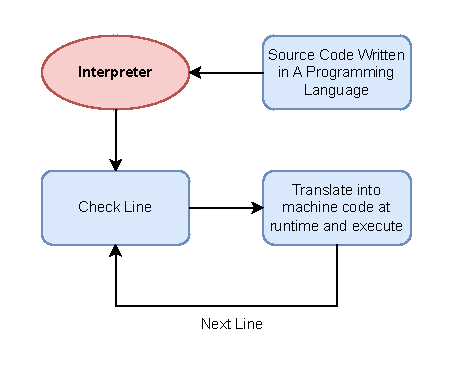
\includegraphics[width=0.5\textwidth]{Chapters/Diagram/Intro/inter.drawio.pdf}
\end{center}

\begin{prettyBox}{Note}{red}
    \textbf{\underline{Pros of an Interpreter}:}
    \begin{itemize}
        \item \textbf{Easier Debugging}: Errors are detected as the program runs, making it easier to pinpoint and fix issues.
        \item \textbf{Platform Independence at Source Level}: The same source code can be executed on different systems without recompilation, as long as an interpreter is available.
        \item \textbf{Smaller Program Size}: Interpreted programs do not require large binary files, reducing storage needs.
    \end{itemize}
    
    \textbf{\underline{Cons of an Interpreter}:}
    \begin{itemize}
        \item \textbf{Slower Execution}: Since interpretation and execution happen simultaneously, it is slower compared to compiled programs.
        \item \textbf{Runtime Errors}: Errors only appear when execution reaches the faulty line, which can lead to unexpected crashes.
    \end{itemize}
\end{prettyBox}

\vspace{0.25cm}
\section{Steps of Compilation}
\begin{prettyBox}{Steps}{myblue}
The process of compilation is done following these steps chronologically:
\begin{enumerate}
    \item Lexical Analysis
    \item Syntactic Analysis (Parsing)
    \item Semantic Analysis
        \begin{itemize}
            \item Generation of Intermediate Code
            \item Syntax-Directed Translation
        \end{itemize}
    \item Generation of Object Code
\end{enumerate}
\end{prettyBox}

\vspace{0.25cm}

\subsection{Lexical Analysis}
\begin{prettyBox}{Lexical Analysis}{myblue}
Lexical analysis consists of dividing the entire code into lexical entities (tokens) storing them in a dictionnary and evaluating each of them independently throught automata or regex. Tokens can be divided based on:
\begin{itemize}
    \item Spaces
    \item Logical operators (AND, OR, NOT, \(>\)=, \(>\), \(<\)=, \(<\), =)
    \item Arithmetic operators (+, -, *, /)
    \item Separators ([ ], \{ \}, ( ))
\end{itemize}
\end{prettyBox}

\newpage
\underline{\textbf{Example}}

\begin{center}
    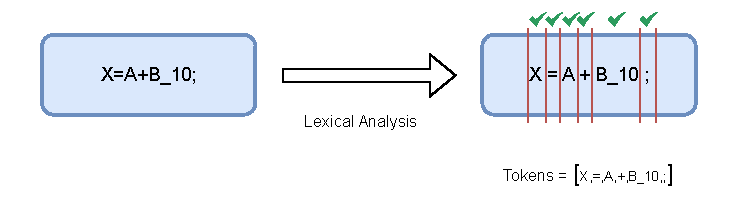
\includegraphics{Chapters/Examples/Intro/ex1.drawio.pdf}
\end{center}

\vspace{0.25cm}
\begin{center}
    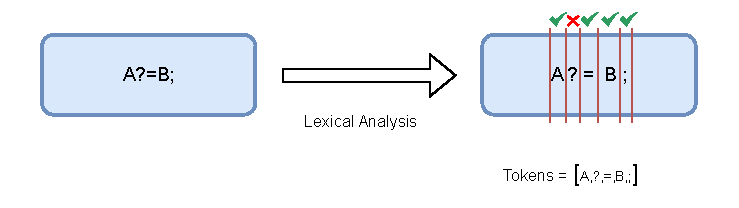
\includegraphics{Chapters/Examples/Intro/ex2.drawio.pdf}
\end{center}

\vspace{0.35cm}

\subsubsection{Types Of Token}
\begin{prettyBox}{Types}{myblue}
\begin{itemize}
    \item \textbf{Constant}: Represent literal values like numbers : (3.14 , 1021 ,-120)  , literal string : "hello world !" and character 'a'.  
    \item \textbf{Keyword}:  Reserved words that have a predefined meaning in the language, like `if`, `while`, and `return`.  
    \item \textbf{Identifier}: Names given to variables, functions, or objects.  
    \item \textbf{Separator}: Symbols used to separate tokens (logical , arithmetic operators ...etc) 
\end{itemize}
\end{prettyBox}

\vspace{0.35cm}


\subsubsection{Automata}
\begin{prettyBox}{Automata}{myblue}
Lexical analysis uses a finit deterministc automata to verify wether a given token is correct or no , a token
is considered correct if it reaches an end state with no blockage in the process
\end{prettyBox}

\newpage
\null

\textbf{\underline{Example}}

\vspace{0.5cm}

\hspace{5.7cm}    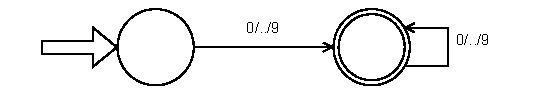
\includegraphics{Chapters/Examples/Intro/ex4.1.drawio.pdf}


\vspace{0.85cm}

 \hspace{5.65cm}   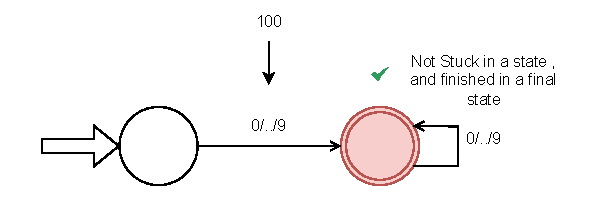
\includegraphics{Chapters/Examples/Intro/ex4.2.drawio.pdf}

\vspace{0.85cm}

 \hspace{5.65cm}   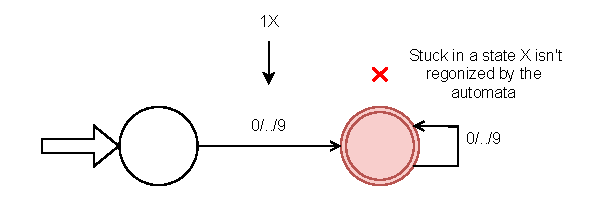
\includegraphics{Chapters/Examples/Intro/ex4.3.drawio.pdf}

\vspace{0.85cm}
  \hspace{5.65cm}  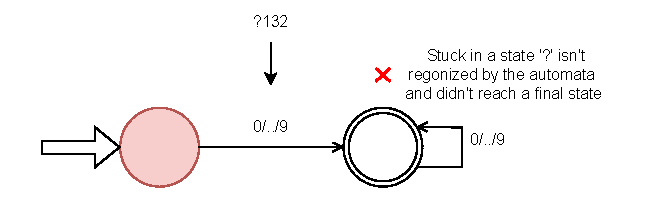
\includegraphics{Chapters/Examples/Intro/ex4.4.drawio.pdf}


\vspace{0.85cm}


\begin{prettyBox}{Note}{red}
Never loop on the start state, as this will always cause undesired behavior, potentially leading to unexpected results or halting the automaton from transitioning to the next valid state.
\end{prettyBox}


\subsection{Syntactic Analysis (Parsing)}
\begin{prettyBox}{Syntactic Analysis}{myblue}
Syntactic analysis checks if the order of tokens is correct and adheres to the required format (using automata or regular expressions).  
There are two methods:  
\begin{itemize}
    \item Descending methods  
    \item Ascending methods  
\end{itemize}
\end{prettyBox}

\vspace{0.95cm}
\underline{\textbf{Example}}

\vspace{0.35cm}
\begin{center}
    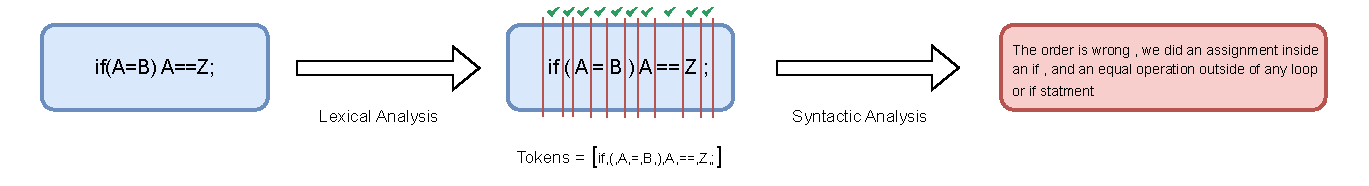
\includegraphics[height=0.14\textheight,width=0.9\textwidth]{Chapters/Examples/Intro/ex3.drawio.pdf}
\end{center}

\vspace{0.5cm}

\begin{prettyBox}{Note}{red}
If a code is lexically correct, it does not guarantee that it will be syntactically correct. However, the opposite is true:

\begin{center}
    Correct Syntactically $\rightarrow$ Correct Lexically \\[0.15cm]
    Correct Lexically $\nrightarrow$ Correct Syntactically
\end{center}

\end{prettyBox}

\vspace{0.35cm}

\subsection{Semantic Analysis}
\begin{prettyBox}{Semantic Analysis}{myblue}
This phase ensures the code is logically correct and adheres to the language's rules. It verifies \textbf{type mismatches, variable declarations, function calls, and more}.

\begin{itemize}
    \item \textbf{Generation of Intermediate Code}: 
    Produces a simplified, platform-independent representation of the program. This step is crucial for optimizing the code and converting it into machine code later , it has many types :
    \begin{itemize}
        \item \textbf{Quadruple Form}
        \item \textbf{Postfix and Prefix Forms ... etc}
    \end{itemize}

    \item \textbf{Syntax-Directed Translation}: 
    Generates intermediate representations, ensuring that the semantics (meaning) of the program guide the creation of subsequent steps.
\end{itemize}
\end{prettyBox}

\vspace{0.35cm}
\subsection{Object Code Generation}

\begin{prettyBox}{Object Code Generation}{myblue}
The final step of compilation, where the object code is generated to execute the program.
This is the only step in the compilation process that we will not cover in this course.
\end{prettyBox}

\vspace{1cm}

\section{Dictionary(Symboles Table)}

\begin{prettyBox}{Dictionary}{myblue}
The dictionary is an array that stores tokens and information about them.
It is first initialized during lexical analysis and then progressively filled
as the analysis continues.
\end{prettyBox}
\vspace{0.35cm}

\begin{center}
    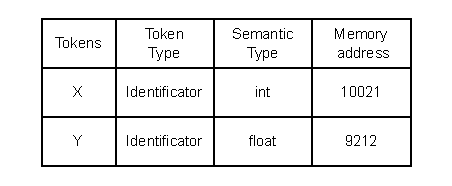
\includegraphics[width=0.6\textwidth]{Chapters/Examples/Intro/dict.drawio.pdf}
\end{center}


\vspace{0.5cm}


\begin{prettyBox}{Note}{red}
Memory allocation occurs after semantic analysis to prevent allocation when
the source code contains errors. This ensures that resources are only allocated
once the code is verified as semantically correct.
\end{prettyBox}

\vspace{0.5cm}

\section{Compilation Steps Diagram}

\vspace{0.3cm}
\begin{center}
    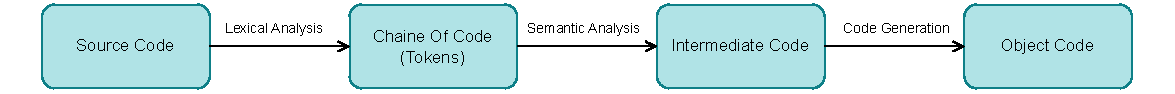
\includegraphics[height=0.08\textheight]{Chapters/Examples/Intro/sum.drawio.pdf}
\end{center}




